\chapter{C++基础}

\section{命名空间}

\subsection{命名空间(namespace)}

多人共同开发时,经常会出现变量和函数定义冲突,例如编写了相同名称的函数。命名空间用于解决这个问题,它可以作为附加信息来区分不同库中的变量和函数。\\

namespace表示了标识符的可见范围,C++标准库中的所有标识符都定义于一个名为std的namespace中。如果不使用using namespace std,就必须使用std::cout、std::endl等表示其中的标识符。\\

\mybox{命名空间}

\begin{lstlisting}[language=C++]
#include <iostream>

namespace foo {
    int n = 123;
    void f() {
        std::cout << "foo::f()" << std::endl;
    }
};

namespace bar {
    int n = 456;
    void f() {
        std::cout << "bar::f()" << std::endl;
    }
};

int main() {
    std::cout << foo::n << std::endl;
    foo::f();
    std::cout << bar::n << std::endl;
    bar::f();
    return 0;
}
\end{lstlisting}

\begin{tcolorbox}
	\mybox{运行结果}
	\begin{verbatim}
123
foo::f()
456
bar::f()
	\end{verbatim}
\end{tcolorbox}

\newpage

\section{重载函数}

\subsection{函数默认参数}

在进行函数参数定义的时候,也可以设置默认值。当参数没有传递的时候就利用默认值来进行参数内容的填充,如果在参数上定义了默认值,那么该参数一定要放在参数列表的最后。\\

\mybox{函数默认参数}

\begin{lstlisting}[language=C++]
#include <iostream>

using namespace std;

void setDate(int year = 1970, int month = 1, int day = 1) {
    cout << year << "/" << month << "/" << day << endl;
}

int main() {
    setDate(2021, 8, 15);
    setDate(2021, 7);
    setDate(2021);
    setDate();
    return 0;
}
\end{lstlisting}

\begin{tcolorbox}
	\mybox{运行结果}
	\begin{verbatim}
2021/8/15
2021/7/1
2021/1/1
1970/1/1
	\end{verbatim}
\end{tcolorbox}

\vspace{0.5cm}

\subsection{重载函数}

重载(overload)表示在同一个作用域中声明了一个与之前声明过的函数具有相同名称的函数,但是它们的参数列表不同。当调用一个重载函数时,编译器通过传递的参数类型,选用最合适的定义。\\

\mybox{重载函数}

\begin{lstlisting}[language=C++]
#include <iostream>
using namespace std;

int max(int num1, int num2) {
    return num1 > num2 ? num1 : num2;
}

double max(double num1, double num2) {
    return num1 > num2 ? num1 : num2;
}

char max(char num1, char num2) {
    return num1 > num2 ? num1 : num2;
}

int main() {
    cout << max(2, 8) << endl;
    cout << max(3.14, 2.71) << endl;
    cout << max('H', 'D') << endl;
    return 0;
}
\end{lstlisting}

\begin{tcolorbox}
	\mybox{运行结果}
	\begin{verbatim}
8
3.14
H
	\end{verbatim}
\end{tcolorbox}

\newpage

\section{引用}

\subsection{引用(Reference)}

在C语言中【\&】表示取地址符,但是在C++中还有引用的特性。引用是指对某一变量的别名,因此引用本身并不占存储单元,对引用的操作与直接对变量的操作完全一样。

\vspace{-0.5cm}

\begin{lstlisting}[language=C++]
data_type &ref_var = var;
\end{lstlisting}

声明引用时必须对其初始化,并且之后不能再将该引用作为其它变量的别名。\\

引用的一个重要作用就是作为函数的参数。C语言中函数参数传递是按值传递,如果有大块数据作为参数传递的时候,往往采用指针的方式,因为这样可以避免将整块数据全部压栈,可以提高程序的效率。但是C++中传递引用给函数与传递指针的效果是一样的,使用引用传递函数的参数,在内存中并没有产生实参的副本,而是直接对实参操作。\\

\mybox{引用}

\begin{lstlisting}[language=C++]
#include <iostream>

using namespace std;

void swap(int& num1, int& num2) {
    int temp = num1;
    num1 = num2;
    num2 = temp;
}

int main() {
    int a = 92;
    int b = 28;
    cout << "Before: " << a << " " << b << endl;
    swap(a, b);
    cout << "After: " << a << " " << b << endl;
    return 0;
}
\end{lstlisting}

\begin{tcolorbox}
	\mybox{运行结果}
	\begin{verbatim}
Before: 92 28
After: 28 92
	\end{verbatim}
\end{tcolorbox}

指针与引用的区别:

\begin{itemize}
	\item 指针有自己的一块空间,而引用只是一个别名,对引用的操作等效于对原变量的操作。

	\item 指针的大小为4或8(根据OS),而引用则是被引用对象的大小。

	\item 指针可以被初始化为NULL,而引用必须被初始化且必须是一个已有对象的引用。

	\item 作为参数传递时,指针需要被解引用才可以对对象进行操作,而直接对引用的修改都会改变引用所指向的对象。

	\item 引用在初始化后,便不能再更改引用的目标。

	\item 指针可以有多级指针,而引用只有一级。

	\item 指针和引用使用【++】运算符的意义不一样。

	\item 返回动态内存分配的内存时必须使用指针,引用可能引起内存泄漏。
\end{itemize}

\newpage

\section{函数指针}

\subsection{函数指针}

函数指针即指向函数的指针,它最大的作用是把一个函数作为参数传递给另外一个函数。在编译时,每一个函数都有一个入口地址,该入口地址就是函数指针所指向的地址。\\

\mybox{函数指针}

\begin{lstlisting}[language=C++]
#include <iostream>

using namespace std;

int add(int num1, int num2) {
    return num1 + num2;
}

int sub(int num1, int num2) {
    return num1 - num2;
}

int get(int num1, int num2, int (*calculate)(int num1, int num2)) {
    return calculate(num1, num2);
}

int main() {
    cout << get(7, 3, add) << endl;
    cout << get(7, 3, sub) << endl;
    return 0;
}
\end{lstlisting}

\begin{tcolorbox}
	\mybox{运行结果}
	\begin{verbatim}
10
4
	\end{verbatim}
\end{tcolorbox}

\vspace{0.5cm}

\subsection{回调函数(Callback Function)}

假设公司要开发一款主打解决国民早餐问题的APP明日油条,为了加快开发进度,这款应用由A小组和B小组协同开发。\\

其中有一个核心模块由A小组开发供B小组调用,这个核心模块被写成了一个函数make\_youtiao()。\\

如果make\_youtiao()执行地很快并可以立即返回,那么B小组只需:

\begin{enumerate}
	\item 调用make\_youtiao()
	\item 等待函数执行完成
	\item 执行后续流程sell()出售
\end{enumerate}

但是现实中make\_youtiao()函数需要处理的数据非常庞大,例如make\_youtiao(10000)不会立刻返回,而是需要等待10分钟才能执行完成。显然直接调用的话,需要等待10分钟后才能继续执行后续代码,这并不是一种高效的做法。\\

因此一种更好的做法是调用make\_youtiao()后不再等待这个函数执行完成,而是让这个函数知道制作完油条后该干什么,例如“制作10000个油条,然后卖出去”。\\

因此make\_youtiao()需要增加一个参数,除了指定制作油条的数量外,还可以指定制作好后该干什么,这个被make\_youtiao()调用的函数就叫回调。\\

\mybox{回调函数}

\begin{lstlisting}[language=C++]
#include <iostream>

using namespace std;

void sell(int n) {
    cout << "selling youtiao ..." << endl;
}

void make_youtiao(int n, void (*sell)(int)) {
    cout << "making youtiao ..." << endl;
    for(int i = 0; i < n; i++);
    sell(n);
}

int main() {
    make_youtiao(10000, sell);
    return 0;
}
\end{lstlisting}

\begin{tcolorbox}
	\mybox{运行结果}
	\begin{verbatim}
making youtiao ...
selling youtiao ...
	\end{verbatim}
\end{tcolorbox}

\newpage

\section{内存管理}

\subsection{malloc() / free()}

C语言使用malloc()分配内存,使用free()释放已分配的内存。当malloc()分配的内存过多/不够时,可以使用realloc()重新分配内存。\\

malloc()的功能是向系统申请指定的内存空间(以字节为单位),使用该函数需要包含头文件stdlib.h。

\vspace{-0.5cm}

\begin{lstlisting}[language=C]
void* malloc(size_t size);
\end{lstlisting}

malloc()的返回值为void *类型,表示一个指向申请到的空间的首地址,是一个无类型的指针,开发者需要自行转换为自己需要的类型。如果malloc()申请内存失败,则会返回空指针NULL。\\

通过malloc()申请来的空间是需要归还给操作系统的,否则程序长时间运行内存会逐渐下降。通过free()可以把申请来的空间释放,但是有两点需要注意:

\begin{enumerate}
	\item 只能释放通过malloc()申请得到的空间。
	\item 只能通过空间的首地址进行释放。
\end{enumerate}

\vspace{0.5cm}

\mybox{malloc() / free()}

\begin{lstlisting}[language=C++]
#include <iostream>
#include <cstdlib>

using namespace std;

int main() {
    const int n = 10;
    int *arr = (int *)malloc(sizeof(int) * n);
    if(!arr) {
        cerr << "Memory allocation failed." << endl;
        return 1;
    }
    for(int i = 0; i < n; i++) {
        arr[i] = i;
        cout << arr[i] << " ";
    }
    cout << endl;
    free(arr);
    return 0;
}
\end{lstlisting}

\begin{tcolorbox}
	\mybox{运行结果}
	\begin{verbatim}
0 1 2 3 4 5 6 7 8 9
	\end{verbatim}
\end{tcolorbox}

\vspace{0.5cm}

\subsection{new / delete}

C++中可以通过new运算符实现动态内存分配,如果空间内配失败,程序则抛出bad\_alloc异常。

\vspace{-0.5cm}

\begin{lstlisting}[language=C++]
T *p = new T;
T *p = new T[N];
\end{lstlisting}

其中T为任意类型名,p是类型为T *的指针。\\

通过new动态内存分配所得的空间在使用完后需要使用delete运算符释放空间。

\vspace{-0.5cm}

\begin{lstlisting}[language=C++]
delete p;
delete[] p;
\end{lstlisting}

如果动态分配new一个数组,但是却用delete释放,而不是delete[],会导致动态分配的数据没有被完全释放。如果动态申请的内存空间不再使用后没有及时释放,就会导致内存泄漏(memory leak)。\\

\mybox{new / delete}

\begin{lstlisting}[language=C++]
#include <iostream>

using namespace std;

int main() {
    int *p1 = new int;
    *p1 = 928;
    cout << "*p1 = " << *p1 << endl;

    const int n = 10;
    int *p2 = new int[n];
    cout << "p2: ";
    for(int i = 0; i < n; i++) {
        p2[i] = i;
        cout << p2[i] << " ";
    }
    cout << endl;

    delete p1;
    delete[] p2;
    return 0;
}
\end{lstlisting}

\begin{tcolorbox}
	\mybox{运行结果}
	\begin{verbatim}
*p1 = 928
p2: 0 1 2 3 4 5 6 7 8 9
	\end{verbatim}
\end{tcolorbox}

\vspace{0.5cm}

\subsection{malloc() / free()与new / delete区别}

\begin{itemize}
	\item new分配内存按照数据类型,而malloc()按照指定指定大小。

	\item new返回指定对象的指针,而malloc()返回void *,因此malloc()的返回值一般都需要类型转换。

	\item new是一个操作符,malloc()是一个库函数。

	\item new分配失败抛出bad\_alloc异常,而malloc()失败返回NULL。
\end{itemize}

\vspace{0.5cm}

\subsection{内存管理}

虚拟内存中栈区的内存是由系统自动分配的,不需要程序员对其进行管理,一般用于存储函数的返回地址、参数、局部变量和返回值。而堆区的内存是动态分配的,并且需要手动释放内存。\\

栈是运行时的单位,堆是存储的单位。栈解决程序运行问题(如何执行),堆解决数据存储的问题(如何存储)。 \\

内存通常包括了栈区(stack)、堆区(heap)、数据区、程序代码区:

\begin{itemize}
	\item 栈区:由编译器自动分配和释放,存放函数的参数值、局部变量的值等。

	\item 堆区:一般由程序员分配和释放,若程序员不释放,程序结束后被OS回收。

	\item 数据区:存放全局变量和静态变量,程序结束后由系统释放。

	\item 程序代码区:存放函数体的二进制代码。
\end{itemize}

\begin{figure}[H]
	\centering
	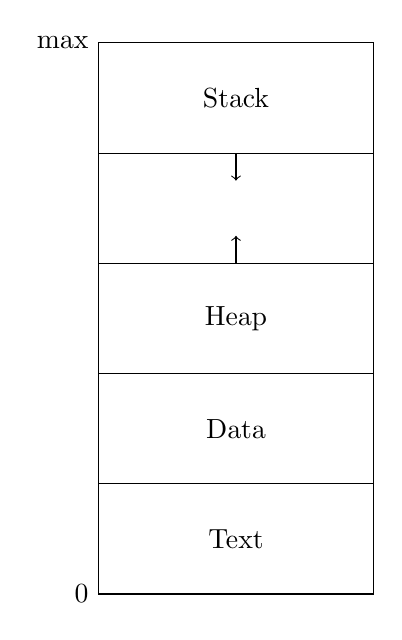
\begin{tikzpicture}[scale=0.7]
		\draw[-] (0,0) -- (0,10) -- (5,10) -- (5,0) -- (0,0);
		\draw[-] (0,2) -- (5,2);
		\draw[-] (0,4) -- (5,4);
		\draw[-] (0,6) -- (5,6);
		\draw[-] (0,8) -- (5,8);

		\draw (0,0) node[left] {0};
		\draw (0,10) node[left] {max};

		\draw (2.5,1) node {Text};
		\draw (2.5,3) node {Data};
		\draw (2.5,5) node {Heap};
		\draw (2.5,9) node {Stack};

		\draw[->] (2.5,8) -- (2.5,7.5);
		\draw[->] (2.5,6) -- (2.5,6.5);
	\end{tikzpicture}
	\caption{内存管理}
\end{figure}

\newpage